\item What is the minimum acceleration with which bar \( A \) (Fig. 1.22) should be shifted horizontally to keep bodies \( 1 \) and \( 2 \) stationary relative to the bar? The masses of the bodies are equal, and the coefficient of friction between the bar and the bodies is equal to \( k \). The masses of the pulley and the threads are negligible, the friction in the pulley is absent.
    \begin{center}
        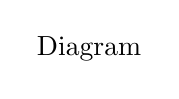
\begin{tikzpicture}
            \node at (0, 0) {Diagram};
        \end{tikzpicture}
    \end{center}
\begin{solution}
    \begin{center}
        \begin{tikzpicture}
            \pic at (0, 0) {frame=3cm};
        \end{tikzpicture}
    \end{center}
    
    % \begin{align*}
    %     \intertext{Bodies 1 and 2 will remain at rest with respect to bar 4 for $w_{\min} \le w \le w_{\max}$ where $w_{\min}$ is the sought minimum acceleration of the bar. Beyond these limits there will be a relative motion between bar and the bodies. For $0 \le w \le w_{\min}$ the tendency of body 1 in relation to the bar A is to move towards right and is in the opposite sense for $w \ge w_{\max}$. On the basis of above argument the static friction on 2 by A is directed upward and on 1 by A is directed towards left for the purpose of calculating $w_{\min}$.}
    %     \intertext{Let us write Newton's second law for bodies 1 and 2 in terms of projection along positive $x$-axis (see figure).}
    %     T - f_{r1} &= mw \quad \text{or} \quad f_{r1} = T - mw \tag{1} 
    %     \intertext{As body 2 has no acceleration in vertical direction, so}
    %     N_2 &= mw \tag{2}
    %     f_{r2} &= mg - T \tag{3}
    %     \intertext{From Eqs. (1) and (3)}
    %     (f_{r1} + f_{r2}) &= m (g - w) \tag{4}
    %     \intertext{But,}
    %     f_{r1} + f_{r2} &\le k (N_1 + N_2) \\
    %     \intertext{or}
    %     f_{r1} + f_{r2} &\le k (mg + mw) \tag{5}
    %     \intertext{From Eqs. (4) and (5)}
    %     m (g - w) &\le mk (g + w) \quad \text{or} \quad w \ge \dfrac{g (1-k)}{1+k} \\
    %     \intertext{Hence,}
    %     w_{min} &= \dfrac{g (1-k)}{1+k}
    % \end{align*}
\end{solution}
